\documentclass[a4paper,dvipsnames]{article}

\input ../../header

\usepackage{minted}
\usepackage{bookmark}
\usepackage{hyperref}
\hypersetup{
  colorlinks=true,
  linkcolor=blue,
  urlcolor=blue,
}
\usepackage{dirtree}

%\newcounter{activite}
%\newcommand{\activite}{\stepcounter{activite}\bigskip\noindent\textbf{Activité \theactivite}\smallskip\hrule\medskip}

\setlength{\multicolsep}{2pt}

\definecolor{bg}{rgb}{0.95,0.95,0.95}

\begin{document}

\title{Projet -- Sapin de Noël (activité 5)}

\pagestyle{empty}

\author{}

\date{}

\maketitle{}

\thispagestyle{empty}

%\section{Interactions Humain-Machine sur le web}
%Les Interactions Humain-Machine (IHM) (on trouve aussi parfois Interfaces Humain-Machine) sur le web définissent les moyens et les outils mis en oeuvre afin qu'une personne physique puisse agir (contrôler, communiquer) à distance, par l'intermédiaire d'Internet par exemple. Parmi ces moyens, on trouve le langage HTML.
%
%\subsection{Le langage HTML}
%Un document HTML est composé de deux parties séparées par des \textit{balises} :
%\begin{itemize}
%  \item son \textit{en-tête}, entre les balises \mintinline{html}{<head>} et \mintinline{html}{</head>} ;
%  \item son \textit{corps}, entre les balises \mintinline{html}{<body>} et \mintinline{html}{</body>}.
%\end{itemize}
%
%Un document HTML ressemble à ceci :
%
%\begin{minted}[bgcolor=bg]{html}
%<!DOCTYPE html>
%<html>
%
%<head>
%    <meta charset="utf-8">
%    <title>Mon titre</title>
%</head>
%
%<body>
%
%</body>
%
%</html>
%\end{minted}
%
%\bigskip
%
%\activite
%\begin{enumerate}
%  \item Télécharger le dossier \og{}Projet sapin\fg{} puis ouvrir le fichier \verb|index.html| dans Atom et dans Firefox.
%  \item Ajouter la ligne suivante dans l'en-tête du fichier HTML :
%\begin{minted}[bgcolor=bg]{html}
%<link rel="icon" href="christmas_tree_favicon.ico">
%\end{minted}
%Rafraîchir la page ouverte dans Firefox : à quoi cette ligne a-t-elle servi ?
%\item Changer le titre de la page en \og{}Mon beau sapin\fg{}.
%\item Modifier le fichier \verb|index.html| afin que la page HTML ressemble à celle décrite par le fichier\\\verb|page_sans_CSS.pdf|.
%  \begin{itemize}
%    \item les liens CSS, JavaScript et Python pointeront respectivement vers :
%      \begin{center}
%	\url{https://www.w3schools.com/css/default.asp},\\
%	\url{https://www.w3schools.com/js/default.asp},\\
%	\url{https://www.w3schools.com/python/default.asp};
%      \end{center} 
%    \item le lien Raspberry Pi 3 modèle B pointera vers :
%      \begin{center}
%	\url{https://www.raspberrypi.org/products/raspberry-pi-3-model-b/}.
%      \end{center} 
%  \end{itemize}
%\end{enumerate}
%
%\pagebreak
%
%\subsection{CSS}
%Le langage CSS (pour l'anglais \textit{Cascading Style Sheets}) est un langage permettant de définir les propriétés graphiques des éléments HTML constituant une page web.
%
%\bigskip
%
%\activite
%\begin{enumerate}
%  \item Rajouter la ligne suivante dans l'en-tête du fichier HTML :
%    \begin{minted}[bgcolor=bg]{html}
%<link rel="stylesheet" href="style.css" type="text/css">
%    \end{minted}
%    Ouvrir ensuite le fichier \verb|style.css| dans Atom (on gardera le fichier \verb|index.html| ouvert).
%  \item Le langage CSS définit une notion de \textit{sélecteur} qui est un moyen d'identifier à quels éléments s'applique une propriété. Écrire les lignes suivantes dans le fichier \verb|style.css| :
%    \begin{minted}[bgcolor=bg]{css}
%body {
%    font-family: sans-serif;
%}
%    \end{minted}
%    Quel effet ces lignes ont-elles produit ?\\
%    \textit{Vocabulaire. -- On dit que \mintinline{css}{body} est un sélecteur. \mintinline{css}{font-family} est une propriété CSS et \mintinline{css}{sans-serif} est sa valeur.}
%  \item Changer la couleur des titres de niveau 1 à l'aide des lignes suivantes :
%    \begin{minted}[bgcolor=bg]{css}
%h1 {
%    color: #B3000C;
%}
%    \end{minted}
%    \textit{Remarque. -- La couleur est donnée en utilisant la notation hexadécimale.}
%  \item Changer également la couleur des titres de niveau 2 (couleur : \mintinline{css}{FF0012}) et celle du contenu des balises \mintinline{html}{strong} (couleur : \mintinline{css}{green}).
%  \item Afin que le mot \og{}interfaces\fg{} ait une autre couleur, on utilise un identifiant. Remplacer la partie :
%
%    \begin{minted}[bgcolor=bg]{html}
%<strong>interfaces</strong>
%    \end{minted}
%
%    par : 
%
%    \begin{minted}[bgcolor=bg]{html}
%<strong id="interfaces">interfaces</strong>
%    \end{minted}
%
%    puis ajouter, dans le fichier CSS :
%    \begin{minted}[bgcolor=bg]{css}
%#interfaces {
%    color: #058A5F;
%}
%    \end{minted}
%    \textit{Vocabulaire. -- On dit que \mintinline{html}{interfaces} est un identifiant.}
%  \item Modifier l'apparence et le comportement des liens hypertextes à l'aide de :
%    \begin{minted}[bgcolor=bg]{css}
%a {
%    color: #B3000C;
%}
%    \end{minted}
%
%    puis de :
%
%    \begin{minted}[bgcolor=bg]{css}
%a:hover {
%    color: #D8D8D8;
%}
%    \end{minted}
%  \item Modifier l'apparence des listes en ajoutant les lignes suivantes :
%    \begin{minted}[bgcolor=bg]{css}
%ul {
%    list-style-image: url(boule.ico);
%}
%    \end{minted}
%
%    \pagebreak
%
%  \item Ajouter une classe à la première image en remplaçant la ligne :
%    \begin{minted}[bgcolor=bg]{html}
%<img src="raspberry_pi.jpg" alt="un Raspberry Pi">
%    \end{minted}
%
%    en :
%
%    \begin{minted}[bgcolor=bg]{html}
%<img src="raspberry_pi.jpg" alt="un Raspberry Pi" class="images">
%    \end{minted}
%
%    Ajouter alors la même classe à la deuxième image puis modifier l'apparence des deux images de la page à l'aide des lignes :
%
%    \begin{minted}[bgcolor=bg]{css}
%.images {
%    width: 20%;
%}
%    \end{minted}
%
%    La déclaration \mintinline{css}{width: 20%;} est appliquée à tous les éléments ayant pour classe \mintinline{html}{images}.
%
%    \bigskip
%
%    \textbf{Remarque importante. -- Dans un fichier HTML, un identifiant est unique alors que plusieurs éléments peuvent avoir la même classe.}
%    
%    \bigskip
%
%  \item Modifier l'apparence des boutons grâce aux lignes :
%    \begin{minted}[bgcolor=bg]{css}
%input {
%    background-color: green;
%    color: white;
%    border: solid;
%    padding: 15px 32px;
%}
%    \end{minted}
%  \item Dans le fichier HTML, où faut-il rajouter la classe \mintinline{html}{boite-flex} pour modifier l'emplacement des boutons à l'aide des lignes suivantes ?
%    \begin{minted}[bgcolor=bg]{css}
%.boite-flex {
%    display: flex;
%    justify-content: center;
%}
%    \end{minted}
%    Le faire puis écrire les lignes précédentes dans le fichier CSS.
%  \item Les propriétés CSS \mintinline{css}{margin-left}, \mintinline{css}{margin-right}, \mintinline{css}{margin-top} et \mintinline{css}{margin-bottom} permettent d'ajouter des marges. Ajouter :
%    \begin{itemize}
%      \item une marge à gauche de \mintinline{css}{30px} aux titres de niveau 1;
%      \item une marge à gauche de \mintinline{css}{60px} aux titres de niveau 2;
%      \item une marge à gauche et une marge à droite de \mintinline{css}{60px} à chaque paragraphe;
%      \item une marge à gauche et une marge à droite de \mintinline{css}{80px} à chaque liste;
%      \item une marge en haut et une marge en bas de \mintinline{css}{10px} à chaque image.
%    \end{itemize}
%\end{enumerate}

%\pagebreak
%
%\subsection{Le langage JavaScript}
%JavaScript est l'un des langages les plus importants du web. Il est principalement utilisé pour gérer l'interactivité dans un navigateur web (côté client) mais peut également être utilisé côté serveur via la plateforme NodeJS.
%
%\bigskip
%

%\setcounter{activite}{2}
%\activite
%\begin{enumerate}
%  \item Dans le dossier \verb|Projet_sapin| créer le dossier \verb|js|, puis créer à l'intérieur de ce dossier le fichier \verb|script.js|. L'arborescence du projet doit ressembler à ceci : 
%
%    \begin{center}
%      \fbox{
%	\begin{minipage}{8cm}
%	  \dirtree{%
%	    .1 /Projet\_sapin.
%	    .2 index.html.
%	    .2 page\_sans\_CSS.pdf.
%	    .2 /css.
%	    .3 style.css.
%	    .2 /img.
%	    .3 boule.ico.
%	    .3 christmas\_tree\_favicon.ico.
%	    .3 raspberry\_pi.jpg.
%	    .3 relais.jpg.
%	    .2 /js.
%	    .3 script.js.
%	  }
%      \end{minipage}}
%    \end{center}
%    Mettre à jour, dans \verb|index.html|, les liens vers le fichier \verb|style.css| et les images et icônes (\verb|boule.ico|, \verb|christmas_tree_favicon.ico|, \verb|raspberry_pi.jpg| et \verb|relais.jpg|).
%  \item Ouvrir le fichier \verb|index.html| dans Firefox et le fichier \verb|script.js| dans Atom.
%    \begin{enumerate}
%      \item Ajouter le code suivant dans le fichier \verb|script.js| : 
%
%    \begin{minted}[bgcolor=bg]{javascript}
%function Bouton_ascendant() {
%     alert("Bouton ascendant cliqué ! ");
%  }
%	\end{minted}
%
%      \item Afin d'appeler la fonction \mintinline{javascript}{Bouton_ascendant()} dans le fichier \verb|index.html|, ajouter dans le fichier \verb|index.html|, avant la balise \mintinline{html}{</body>} la ligne suivante : 
%
%	\begin{minted}[bgcolor=bg]{html}
%<script type="text/javascript" src="./js/script.js"></script>
%	\end{minted}
%
%	\textit{On prendra l'habitude de placer le code JavaScript en fin de page HTML plutôt qu'entre les balises \mintinline{html}{<head>}}.
%
%	\medskip
%
%	Modifier la ligne : 
%
%	\begin{minted}[bgcolor=bg]{html}
%<input type="button" value="Ascendant" />
%	\end{minted}
%
%	en : 
%
%	\begin{minted}[bgcolor=bg]{html}
%<input type="button" value="Ascendant" onclick="Bouton_ascendant();" />
%	\end{minted}
%
%      \item Rafraîchir la page \verb|index.html|, puis cliquer sur le bouton \og{}Ascendant\fg{}. Que se passe-t-il ? 
%      \item Modifier le fichier \verb|script.js| en remplaçant l'instruction : 
%
%	\begin{minted}[bgcolor=bg]{javascript}
%alert("Bouton Ascendant cliqué ! ");
%	\end{minted}
%
%	en :
%
%	\begin{minted}[bgcolor=bg]{javascript}
%console.log("Bouton Ascendant cliqué ! ")
%	\end{minted}
%
%	Rafraîchir la page \verb|index.html|, puis cliquer sur le button \og{}Ascendant\fg. Que se passe-t-il ?
%      \item Dans Firefox, ouvrir la \verb|Console Web| : \verb|Outils > Développement Web > Console Web|. Qu'observe-t-on ?
%    \end{enumerate}
%
%    \pagebreak 
%
%  \item Afin de pouvoir interagir avec le serveur, nous allons envoyer une requête \verb|GET| au serveur pour qu'il exécute la commande associée au bouton cliqué. 
%    \begin{enumerate}
%      \item Ajouter à la fonction \mintinline{javascript}{Bouton_ascendant()} du fichier \verb|script.js| les lignes suivantes : 
%
%	\begin{minted}[bgcolor=bg]{javascript}
%var request = new XMLHttpRequest(); //Initialisation 
%request.open("GET", "/Ascendant"); //Création de la requête GET
%request.send(); //Envoi de la requête GET au serveur
%	\end{minted}
%
%	\textit{La requête GET ne va pas aboutir pour le moment puisque le serveur web n'a pas été mis en place.}
%
%	Quelle erreur obtient-on dans la \verb|Console Web| lorsqu'on clique sur le bouton \og{}Ascendant\fg{} ?
%      \item Écrire une fonction pour chacun des boutons de la page web : 
%
%	\begin{center}\mintinline{javascript}{Bouton_descendant()}, \mintinline{javascript}{Bouton_alterne()} et \mintinline{javascript}{Bouton_aleatoire()}. 
%	\end{center}
%
%	Ces fonctions, enverront respectivement les requêtes GET :
%
%	\begin{center}
%	  \mintinline{javascript}{"/Descendant"}, \mintinline{javascript}{"/Alterné"} et \mintinline{javascript}{"/Aléatoire"}.
%	\end{center}
%
%	Modifier le fichier \verb|index.html| en conséquence. {\itshape On vérifiera que les boutons envoient bien un message, dans la \verb|Console Web|, confirmant que le clic a bien été pris en compte.}
%    \end{enumerate}
%  \item Écrire en commentaire une description de la fonction \mintinline{javascript}{Bouton_ascendant()}.
%\item Rechercher la définition des requêtes HTTP de type \verb|GET| et \verb|POST|, ainsi que leur utilité.
%\item {\itshape Facultatif. -- On utilise ici 4 fonctions faisant presque la même action : envoyer une requête \verb|GET| constituée d'une action à effectuer sur les guirlandes lumineuses.
%  Il est possible d'écrire une seule fonction en récupérant la valeur du paramètre \mintinline{javascript}{value} du bouton avec l'instruction \mintinline{javascript}{event.target.value}\\
%Effectuer les modifications nécessaires dans les fichiers \verb|script.js| et \verb|index.html| pour \og{}factoriser\fg{} votre code.}
%\end{enumerate}
%
%\pagebreak
%
%\setcounter{section}{1}
%\section{Interaction client/serveur}
%
%\textbf{Rappels}
%
%\begin{itemize}
%\item Le logiciel serveur offre un service sur le réseau. Le serveur accepte des requêtes, les traite et envoie le résultat au demandeur.
%\item Le logiciel client utilise le service offert par le logiciel serveur. Le client envoie des requêtes et reçoit des réponses.
%\end{itemize}
%
%\begin{center}
%  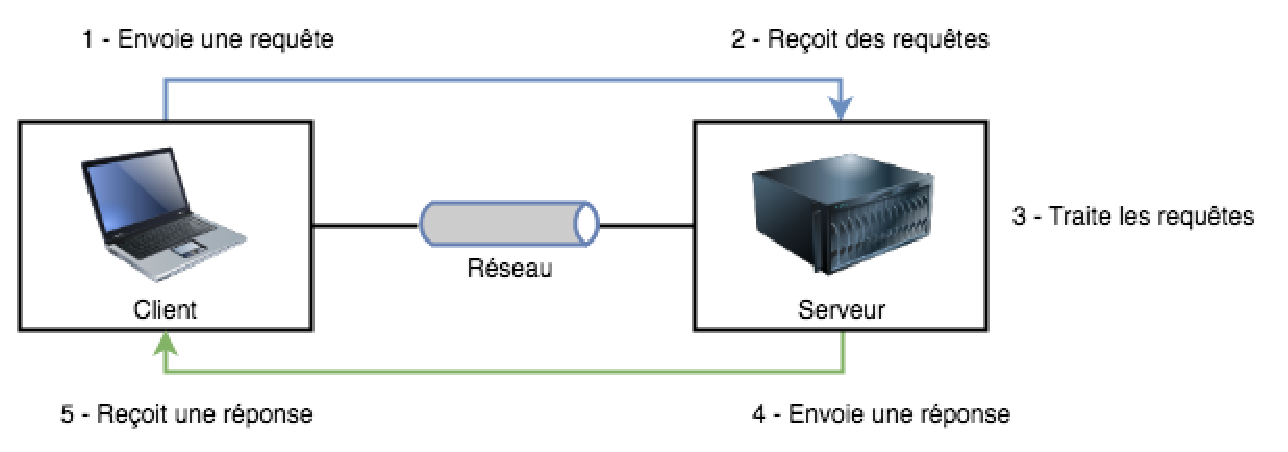
\includegraphics[width=14.5cm]{images/tex/client-serveur.eps}
%\end{center} 
%
%\setcounter{activite}{3}
%
%\activite
%\begin{enumerate}
%  \item Dans le dossier \verb|Projet_sapin| créer les dossiers \verb|templates| et \verb|static| puis créer le fichier \verb|app.py| afin de reproduire l'arborescence ci-dessous : 
%
%    \begin{center}
%      \fbox{
%	\begin{minipage}{8cm}
%	  \dirtree{%
%	    .1 /Projet\_sapin.
%	    .2 app.py.
%	    .2 page\_sans\_CSS.pdf.
%	    .2 /static.
%	    .3 /css.
%	    .4 style.css.
%	    .3 /img.
%	    .4 boule.ico.
%	    .4 christmas\_tree\_favicon.ico.
%	    .4 raspberry\_pi.jpg.
%	    .4 relais.jpg.
%	    .3 /js.
%	    .4 script.js.
%	    .2 /templates.
%	    .3 index.html.
%	  }
%      \end{minipage}}
%    \end{center}
%  \item Ouvrir le fichier \verb|app.py| dans VS Code, puis y ajouter les lignes suivantes : 
%
%	\begin{minted}[bgcolor=bg]{python}
%#!/usr/bin/python
%# -*- coding: UTF-8
%
%from flask import Flask, render_template
%
%# Initialisation de la méthode
%app = Flask(__name__)
%
%# Gestion du chemin
%@app.route("/", methods=["GET"])
%def affiche_index():
%    return render_template("index.html")
%
%@app.route("/Ascendant", methods=["GET"])
%def action_ascendant():
%    print("Requête GET /Ascendant bien reçue")
%    return ("Succès",200)
%
%# Lancement du serveur web
%if __name__ == "__main__":
%    app.run(host="127.0.0.1", port=5555, debug=True)
%	\end{minted}
%
%    {\itshape La bibliothèque externe \verb|Flask| permet de créer un serveur web en langage Python. Pour en savoir plus : \url{https://flask-doc.readthedocs.io/}.}
%  \item Ouvrir les fichiers \verb|index.html| et \verb|style.css| dans VS Code puis modifier les chemins des ressources. Par exemple :  
%
%	\begin{minted}[bgcolor=bg]{html}
%<link rel="stylesheet" href="./css/style.css" type="text/css" />
%	\end{minted}
%
%    devient : 
%
%	\begin{minted}[bgcolor=bg]{html}
%<link rel="stylesheet" href="./static/css/style.css" type="text/css" />
%    \end{minted}
%  \item Activer l'environnement virtuel en écrivant la commande \verb|env_python| dans le terminal, puis lancer le script \verb|app.py| avec la commande \verb|python app.py|.
%  \item Ouvrir un navigateur web et écrire l'adresse \url{http://localhost:5555}. 
%    \begin{enumerate}
%      \item Dans Firefox, ouvrir la \verb|Console Web| puis cliquer sur le bouton \og{}Ascendant\fg. Que constate-t-on ?
%      \item Dans le terminal, d'où le fichier \verb|app.py| a été lancé, que constate-t-on ?
%    \end{enumerate}
%  \item
%
%    \begin{enumerate}
%      \item Reprendre la question 5. avec l'adresse \url{http://127.0.0.1:5555}.  Quelle est la différence entre les deux adresses utilisées ? 
%      \item À quoi sert le nombre \verb|5555| ajouté à la fin de l'adresse ? 
%    \end{enumerate}
%  \item Ajouter les routes correspondant aux différentes requêtes \verb|GET| construites dans l'activité 3 puis vérifier que les actions sont bien prises en compte côté client et côté serveur.
%  \item {\itshape Les 4 routes construites, correspondant aux actions à exécuter sur les guirlandes lumineuses, sont très similaires. Il est possible de faire passer en variable la commande de la requête en écrivant :
%    \begin{center}
%      \mintinline{python}{@app.route('/<command>', methods=['GET'])}
%    \end{center} 
%et d'insérer la variable \mintinline{python}{command} comme paramètre dans la fonction associée à la route.\\ Effectuer les modifications nécessaires dans le fichier \verb|app.py| pour \og factoriser \fg{} votre code.}
%\end{enumerate}
%
%\pagebreak
\setcounter{section}{2}
\subsection{Le matériel utilisé}

Le projet nécessite le matériel suivant :

\begin{itemize}
  \item un Raspberry Pi 3 modèle B;
  \item un module à relais;
  \item un sapin et des guirlandes !
\end{itemize}

\bigskip

Le Raspberry Pi est un \og{}nano-ordinateur\fg{} créé à l'origine pour favoriser l'apprentissage du langage informatique. Pour ce projet, on utilisera le Raspberry Pi 3 B avec la distribution GNU/Linux Raspbian (déjà installée).

\bigskip

\begin{activite}[breakable,title=Activité 5]{}{}
  Retrouver les principales caractéristiques du Raspberry Pi 3 B et identifier les principaux composants de la carte.

  \bigskip

  Le Raspberry Pi 3 B dispose en particulier de 40 broches (ou ports) GPIO (de l'anglais \textit{General Purpose Input/Output}) dont la plupart (voir le schéma ci-dessous) peuvent être utilisées aussi bien en entrée qu'en sortie. Pour ce projet, on utilisera le module Python \verb|gpiozero| permettant de contrôler ces broches.

  \begin{center}
    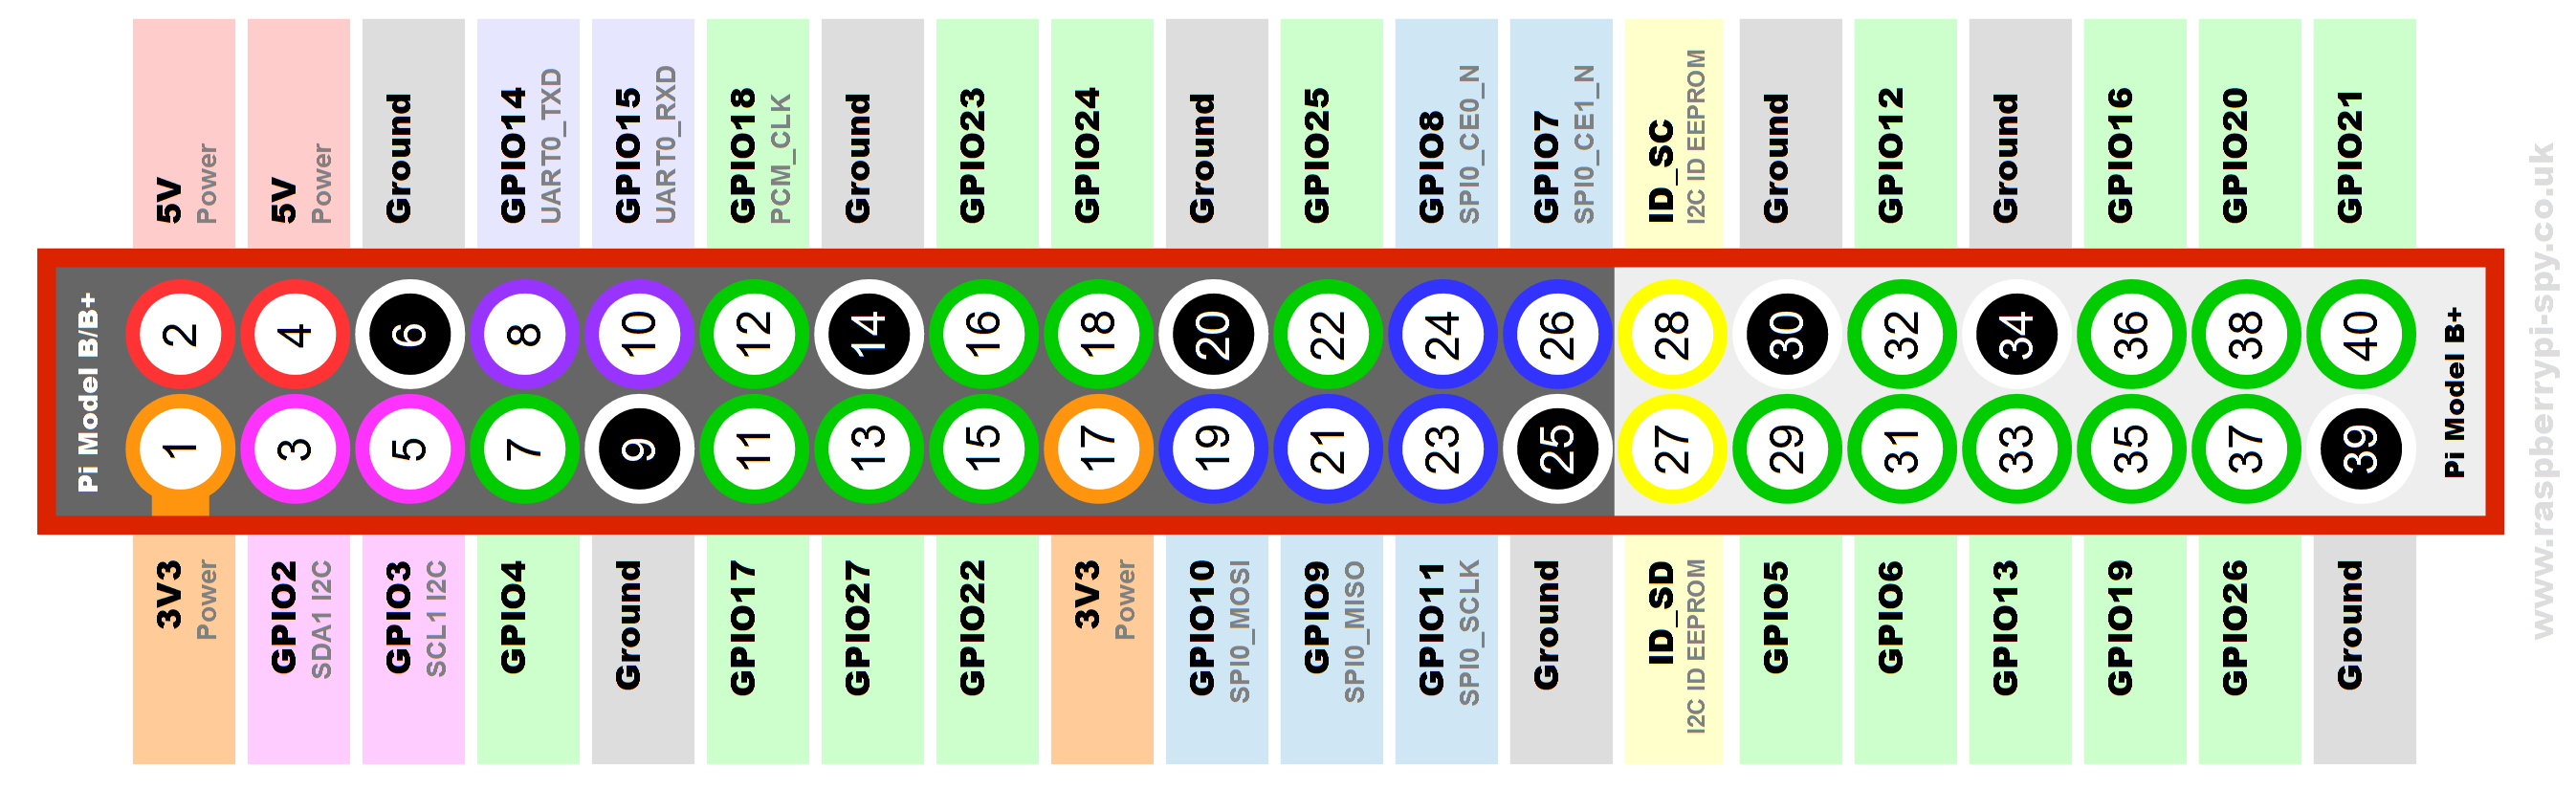
\includegraphics[width=15cm]{images/tex/gpio.png}
  \end{center}

  Le projet nécessite également l'utilisation d'un module à relais comme celui présenté ci-dessous :

  \begin{center}
    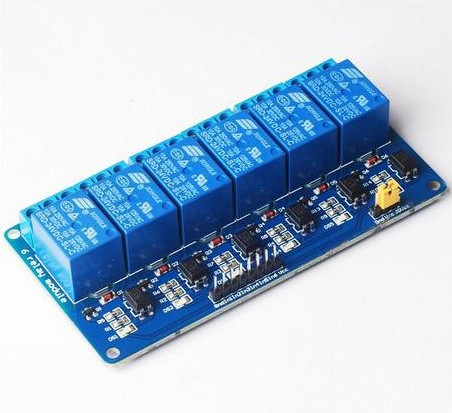
\includegraphics[width=8cm]{images/relais.jpg}
  \end{center}
\end{activite}

%
%\pagebreak
%
%\activite
%\begin{enumerate}
%  \item Réaliser le montage ci-dessous :
%    \begin{center}
%      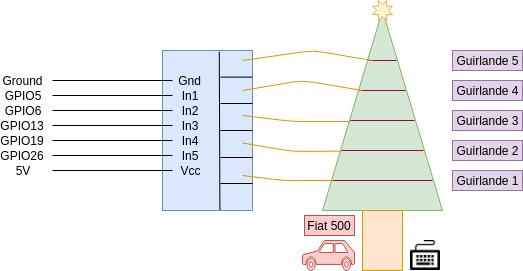
\includegraphics[width=12cm]{images/tex/montage.png}
%    \end{center}
%  \item Dans le dossier \verb|Projet_sapin|, créer un fichier \verb|fonctions_guirlandes.py| dans lequel on écrira les lignes suivantes :
%    \begin{minted}[bgcolor=bg]{python}
%#!/usr/bin/python
%# -*- coding: UTF-8
%
%from gpiozero import OutputDevice
%from time import sleep
%
%guirlande_1 = OutputDevice(26, active_high=False, initial_value=True)
%
%guirlande_1.on()
%sleep(2)
%guirlande_1.off()
%sleep(2)
%    \end{minted}
%    L'arborescence du projet ressemble donc à ceci :
%
%    \begin{center}
%      \fbox{
%	\begin{minipage}{8cm}
%	  \dirtree{%
%	    .1 /Projet\_sapin.
%	    .2 app.py.
%	    .2 fonctions\_guirlandes.py.
%	    .2 page\_sans\_CSS.pdf.
%	    .2 /static.
%	    .3 /css.
%	    .4 style.css.
%	    .3 /img.
%	    .4 boule.ico.
%	    .4 christmas\_tree\_favicon.ico.
%	    .4 raspberry\_pi.jpg.
%	    .4 relais.jpg.
%	    .3 /js.
%	    .4 script.js.
%	    .2 /templates.
%	    .3 index.html.
%	  }
%      \end{minipage}}
%    \end{center}
%  \item Copier le dossier \verb|Projet_sapin| sur le Raspberry Pi (le nom de l'utilisateur par défaut est \verb|pi| et son mot de passe est \verb|raspberry|), puis essayer le script précédent.
%  \item Effacer les lignes précédentes, puis écrire (toujours dans le fichier \verb|fonctions_guirlandes.py|) les fonctions suivantes:
%    \begin{itemize}
%      \item \mintinline{python}{allume_ascendant} qui allume les guirlandes une par une, du bas vers le haut, quatre fois;
%      \item \mintinline{python}{allume_descendant} qui allume les guirlandes une par une, du haut vers le bas, quatre fois;
%      \item \mintinline{python}{allume_alterne} qui allume alternativement les guirlandes de numéro impair et les guirlandes de numéro pair, quatre fois;
%      \item \mintinline{python}{allume_aleatoirement} qui allume deux guirlandes au hasard, les éteint, puis recommence 19 fois.
%    \end{itemize}
%    Chacune des fonctions commencera par éteindre toutes les guirlandes.
%  \item Essayer chacune des fonctions précédentes.
%  \item Apporter les modifications nécessaires pour terminer ce projet.
%\end{enumerate}

\end{document}
